\begin{figure}[H]
    \centering
    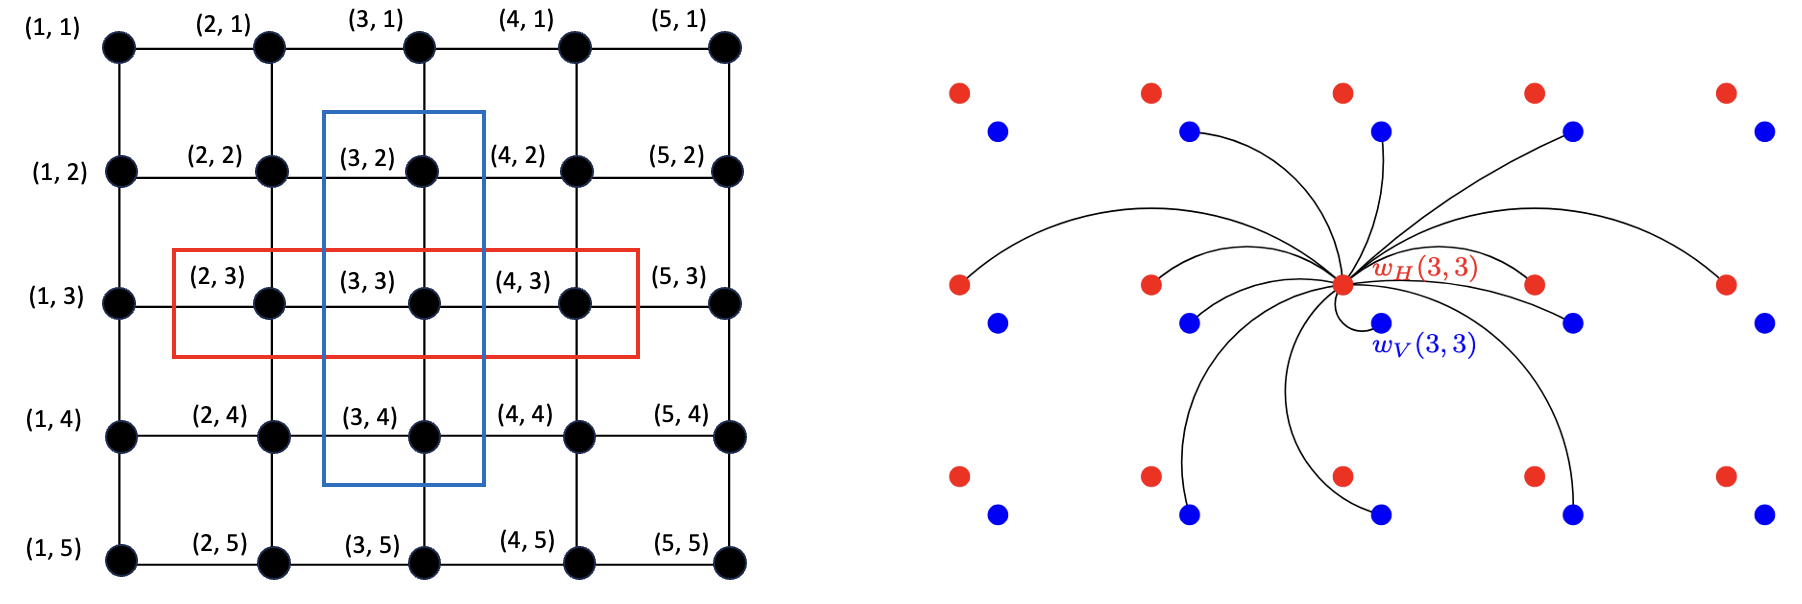
\includegraphics[width=1\linewidth]{cluster-conflict.png}
    % \caption{Example construction of the conflict graph $H$ for a 2D cluster state. Left: a $2\mathrm{D}$ cluster lattice with representative ordered triples centered at interior qubits (e.g., horizontal and vertical triples around $(3,3)$). Right: the local neighborhood of a representative vertex of $H$, showing that each triple conflicts with at most seven others in this construction. Hence $\Delta(H)\le 7$, implying $\chi(H)\le 8$ and therefore at most $2\chi(H)\le 16$ orderings are sufficient to recover all gate-level depolarizing parameters.}

%\input{local_h.pdf_t}

    \caption{Possible construction of the graph $H$ for a 2D cluster-state graph $G$.
      (Top) The black vertices and edges are that of the 2D cluster-state. Qubits are indexed by their coordinates on the grid. The blue and red sets of qubits are the two triples that need to be considered for constructing the graph \(H\) from \(G\) at qubit \((3,3)\). Indeed, at qubit \((3,3)\) there are four \(\lambda\) parameters to estimate, corresponding to the four edges incident to this qubit. Here, each triple infers two different parameters. This being the case for all qubits, the vertices in \(H\) can be partitioned in two sets corresponding to horizontal and vertical triples. ()Bottom) The graph \(H\) constructed around the horizontal triple of qubit \((3,3)\) denoted \(w_H(3,3)\). The vertex \(w_V(3,3)\) corresponds to the vertical triple for qubit \((3,3)\). The other red and blue nodes correspond to the horizontal and vertical triples for the qubits of the graph \(G\). The neighborhood of \(w_H(3,3)\) is made of all triples that share a qubit with it. This amounts to \(w_H(1,3), w_H(2,3), w_H(4,3), w_H(5,3)\) for the horizontal ones and \(w_V(2,2), w_V(2,3), w_V(2,4), w_V(3,2), w_V(3,3), w_V(3,4), w_V(4,2), w_V(4,3), w_V(4,4)\). This shows that the degree of \(w_H(3,3)\) is 13. By symmetry, with periodic boundary conditions on \(G\), all nodes in \(H\) have degree 13. This means that the chromatic number is bounded by 14 and that 28 orderings are enough to gather all possible depolarizing parameters for the 2D cluster state. Only the edges incident to $w_H(3,3)$ have been pictured.}
    \label{fig:2d-cluster}
\end{figure}
